\begin{figure}[htbp]
    \centering
    \resizebox{0.92\textwidth}{!}{%
    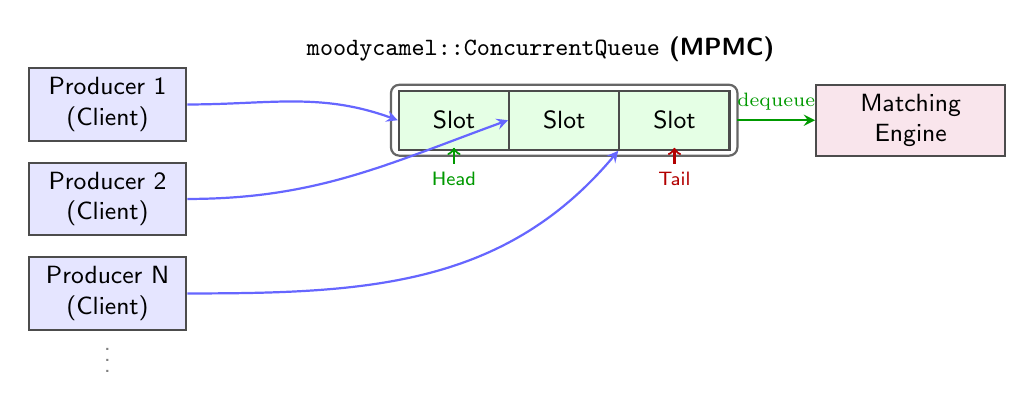
\begin{tikzpicture}[
        font=\sffamily\small,
        producer/.style={
            rectangle, draw=black!70, thick,
            fill=blue!10, minimum width=2.0cm,
            minimum height=0.7cm, align=center
        },
        queuecell/.style={
            rectangle, draw=black!70, thick,
            fill=green!10, minimum width=1.4cm,
            minimum height=0.75cm, align=center
        },
        consumer/.style={
            rectangle, draw=black!70, thick,
            fill=purple!10, minimum width=2.4cm,
            minimum height=0.8cm, align=center
        },
        arr/.style={->, thick, >=stealth}
    ]

    % Producers on left
    \node[producer] (p1) at (0, 2.4) {Producer 1\\(Client)};
    \node[producer] (p2) at (0, 1.2) {Producer 2\\(Client)};
    \node[producer] (p3) at (0, 0.0) {Producer N\\(Client)};

    % Dots between producers
    \node[font=\sffamily\small, text=gray] at (0, -0.75) {\vdots};

    % MPMC Queue label
    \node[font=\sffamily\bfseries\small] at (5.5, 3.1)
        {\texttt{moodycamel::ConcurrentQueue} (MPMC)};

    % Queue cells
    \node[queuecell] (q1) at (4.4, 2.2) {Slot};
    \node[queuecell] (q2) at (5.8, 2.2) {Slot};
    \node[queuecell] (q3) at (7.2, 2.2) {Slot};

    % Queue border
    \draw[black!60, thick, rounded corners=3pt]
        (3.6, 1.75) rectangle (8.0, 2.65);

    % Head / Tail pointer labels
    \node[font=\sffamily\scriptsize, text=green!60!black]
        at (4.4, 1.45) {Head};
    \node[font=\sffamily\scriptsize, text=red!70!black]
        at (7.2, 1.45) {Tail};
    \draw[->, color=green!60!black, thick] (4.4, 1.65) -- (4.4, 1.85);
    \draw[->, color=red!70!black,   thick] (7.2, 1.65) -- (7.2, 1.85);

    % Arrows from producers to queue
    \draw[arr, color=blue!60]
        (p1.east) to[out=0,  in=160] (q1.west);
    \draw[arr, color=blue!60]
        (p2.east) to[out=0,  in=200] (q2.west);
    \draw[arr, color=blue!60]
        (p3.east) to[out=0,  in=230] (q3.south west);

    % Consumer
    \node[consumer] (me) at (10.2, 2.2) {Matching\\Engine};

    % Arrow from queue to consumer
    \draw[arr, color=green!60!black]
        (8.0, 2.2) -- (me.west)
        node[midway, above, font=\scriptsize] {dequeue};

    \end{tikzpicture}%
    }
    \caption{Multi-Producer Multi-Consumer (MPMC) queue contention model.
    Multiple concurrent producer threads (one per trading client) 
    independently push order messages into the shared 
    \texttt{moodycamel::ConcurrentQueue}.
    Atomic Head and Tail indices coordinate access without 
    OS-level locking.
    A single consumer thread (the Matching Engine) dequeues 
    messages sequentially, allowing the system to measure 
    throughput degradation as producer count increases.}
    \label{fig:mpmc_contention}
\end{figure}
